\documentclass[a4paper,german,12pt,smallheadings]{scrartcl}
\usepackage[T1]{fontenc}
\usepackage[utf8]{inputenc}
\usepackage{babel}
\usepackage{geometry}
\usepackage{pdfpages}
\usepackage{tikz}
\usetikzlibrary{calc,intersections,fadings}
\usepackage{wrapfig}
\usepackage[fleqn]{amsmath}
\usepackage{amssymb}
\usepackage{float}
\usepackage{enumerate}
\usepackage{listings} % Source code
\usepackage{lscape} % landscape
\usepackage{commath} % http://tex.stackexchange.com/questions/14821/whats-the-proper-way-to-typeset-a-differential-operator
\usepackage{cancel}
\usepackage[fleqn]{mathtools}
% Number only referenced equations
%\mathtoolsset{showonlyrefs}

%\usepackage{wrapfig}
\usepackage{siunitx}
\sisetup{separate-uncertainty=true,locale=DE}

% http://tex.stackexchange.com/questions/38818/best-way-to-denote-an-angle-in-tikz
\newcommand\markangle[6][red]{% [color] {X} {origin} {Y} {mark} {radius}
  % filled circle: red by default
  \begin{scope}
    \path[clip] (#2) -- (#3) -- (#4);
    \fill[color=#1,fill opacity=0.5,draw=#1,name path=circle]
    (#3) circle (#6mm);
  \end{scope}
  % middle calculation
  \path[name path=line one] (#3) -- (#2);
  \path[name path=line two] (#3) -- (#4);
  \path[%
  name intersections={of=line one and circle, by={inter one}},
  name intersections={of=line two and circle, by={inter two}}
  ] (inter one) -- (inter two) coordinate[pos=.5] (middle);
  % bissectrice definition
  \path[%
  name path=bissectrice
  ] (#3) -- (barycentric cs:#3=-1,middle=1.2);
  % put mark
  \path[
  name intersections={of=bissectrice and circle, by={middleArc}}
  ] (#3) -- (middleArc) node[pos=1.3] {#5};
  }

% New command for color underlining
\usepackage{xcolor}
\newcommand\invisiblesection[1]{%
    \refstepcounter{section}%
      \addcontentsline{toc}{section}{\protect\numberline{\thesection}#1}%
        \sectionmark{#1}}
\newsavebox\MBox
\newcommand\colul[2][red]{{\sbox\MBox{$#2$}%
  \rlap{\usebox\MBox}\color{#1}\rule[-1.2\dp\MBox]{\wd\MBox}{0.5pt}}}

\restylefloat{table}
\geometry{a4paper, top=15mm, left=20mm, right=10mm, bottom=20mm, headsep=10mm, footskip=12mm}
\linespread{1.5}
\setlength\parindent{0pt}
\DeclareMathOperator{\Tr}{Tr}
\DeclareMathOperator{\Var}{Var}
\begin{document}

\begin{titlepage}
\newcommand{\HRule}{\rule{\linewidth}{0.5mm}}

\begin{center}
  \textsc{\Large Physikalisches Grundpraktkum 1}
  \HRule\\[0.4 cm]
  {\huge \bfseries Gleichmäßig beschleunigte Drehbewegungen}
  \HRule\\[0.4 cm]

  \begin{minipage}{0.65\textwidth}
  \begin{flushleft}
    Markus Fenske \texttt{<iblue@zedat.fu-berlin.de>} \\
    Paul Rahmann \texttt{<paulrahmann@zedat.fu-berlin.de>}
  \end{flushleft}
  \end{minipage}
  \hfill
  \begin{minipage}{0.30\textwidth}
  \begin{flushright}
    Tutor: Christian Hindermann \\
    Versuchstag: 6. Juni 2014
  \end{flushright}
  \end{minipage}

  \vspace{1cm}

  \tableofcontents


  %{\large \today}
  \vfill
\end{center}
\newpage

\end{titlepage}

\allowdisplaybreaks % Seitenumbrüche in Formeln erlauben

\section{Physikalische Grundlagen}
\subsection{Herleitung der Bewegungsgleichungen}

Gegeben seien 4 parallele stabförmige (exakter: mit hyperbolischem Querschnitt) Elektroden die jeweils zu ihrem Nachbarn
eine zeitabhängige Potentialdifferenz aufweisen, aber zu ihrem
gegenüberliegenden Nachbarn potentialneutral seien (Quadrupol-Konfiguration)
und jeweils kreuzweise gegenüberliegend den Abstand $2r_0$ voneinander haben.
Wir bestimmen die Bewegungsgleichungen eines Ions zwischen den Stäben.

Aus der Definition des elektrischen Feldes durch das Potential
($\vec{E} = - \nabla \Phi(\vec{r})$) und der ersten Maxellschen Gleichung
($\nabla \vec{E}(\vec{r}) = \rho(\vec{r}) / \epsilon_0$) folgt für den ladungsfreien
Raum ($\rho = 0$) direkt die Poissongleichung

\begin{equation}
  \Delta \Phi(\vec{r}) = 0
\end{equation}

Wir betrachten das Potential in dieser Konfiguration näherungsweise als
Quadrupol-Feld, also gilt
\begin{equation}
  \Phi = \Phi_0 \del{\alpha x^2 + \beta y^2 + \gamma z^2}
\end{equation}

Seien die Elektroden entlang der z-Achse ausgerichtet und näherungsweise
unendlich lang, gibt es in dieser Richtung kein Potential, es gilt also $\gamma
= 0$. Durch Anwendung der Poissiongleichung auf das Potential erhält man
$\alpha = -\beta$. Somit gilt
\begin{equation}
  \Phi = \Phi_0 \alpha \del{x^2 - y^2}
\end{equation}

Das Potetnial bestehe aus einem Gleischspannungsanteil $2U$ und einem zeitabhängigen Wechselfeld $2V \cos(\omega t)$. Dann ergibt sich für das Potential:

\begin{equation}
  \Phi(x,y,t) = \del{U + V \cos(\omega t)} \frac{x^2-y^2}{r_0^2}
\end{equation}

Wir betrachten nun ein Ion der Masse $m$ und Ladung $-q$ zwischen den Stäben.
Aus $\vec{F} = -q E_i = -q \partial_i \Phi$ und $\vec{F} = m \partial_t^2 x_i$
folgen die Bewegungsgleichungen

\begin{align}
  m \frac{\partial^2 x}{\partial t^2} + q \del{U + V \cos(\omega t)} \frac{2 x}{r_0^2} &= 0 \\
  m \frac{\partial^2 y}{\partial t^2} - q \del{U + V \cos(\omega t)} \frac{2 y}{r_0^2} &= 0 \\
  m \frac{\partial^2 z}{\partial t^2} &= 0
\end{align}

Die letzte Differentialgleichung liefert sofort $\dot z=const.$; das Ion bewegt sich also mit konstanter (und meist niedriger) Geschwindigkeit durch den Quadrupol. Für die beiden anderen
betrachten wir die Substitution

\begin{align}
  \omega t &= 2 \xi \left(\Rightarrow \frac{d^2 x}{d \xi^2}=\frac{4}{\omega^2}\frac{\partial^2 x}{\partial t^2} \right) \\
  a &= \frac{8qU}{m r_0^2 \omega^2} \\
  b &= \frac{4qV}{m r_0^2 \omega^2}
\end{align}

und erhalten

\begin{align}
  x'' + (a + 2 b \cos(2 \xi)) x = 0 \\
  y'' - (a + 2 b \cos(2 \xi)) y = 0 
\end{align}

Dies entspricht der Normalform der Mathieuschen Differentialgleichung, deren
Lösungen durch folgende Reihenterme gegeben sind. Wir betrachten hier nur die
$x$-Komponente, die andere Gleichung löst sich analog.

\begin{equation}
  x = \alpha' e^{\mu \xi} \sum_{s=-\infty}^{\infty} c_{2s} e^{2is \xi} + \alpha'' e^{-\mu \xi} \sum_{s=-\infty}^{\infty} c_{2s} e^{-2is \xi}
\end{equation}

Uns interessieren an dieser Stelle nicht die exakten Bewegungen, sondern
interessant ist, ob das Ion in der Falle verbleibt ($|x|$ beschränkt, insbesondere $<r_0$) oder sie
verlässt ($x \to \infty$). Dafür betrachten wir das Zeitverhalten im
Unendlichen ($\xi \to \infty$).

Es existiert $\lim_{\xi \to \infty} e^{\mu \xi}$ genau dann, wenn $\mu = i
\beta$ mit $\beta \in \mathbb{R} \setminus \{0\}$, es gibt also nur in diesem Bereich stabile
Lösungen.

\subsection{Stabilitätsdiagramm}

Die Stabilität der Lösung hängt also nur von $\mu$ und damit von $a$ und $b$
ab, so dass sich unter Zuhilfename der Lösungen für $y$ ein Stabilitäsdiagramm ergibt.

\begin{figure}[H]
  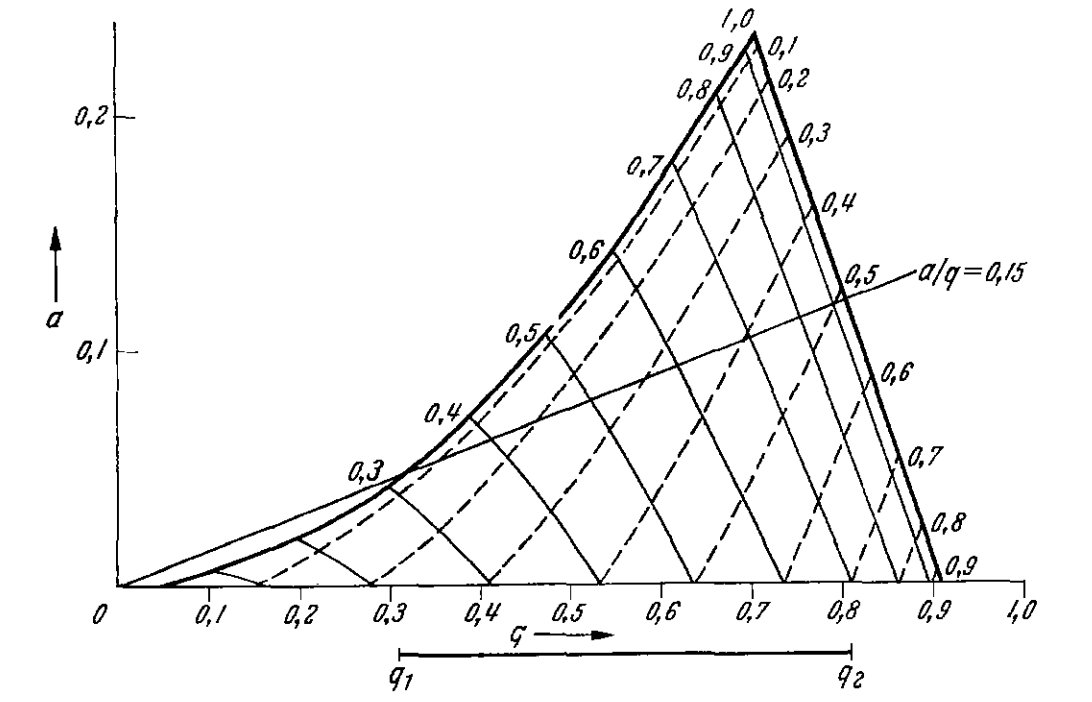
\includegraphics[width=0.7\textwidth]{stabidiag.png}
	\label{stabidiag}
  \caption{Stabilitätsdiagramm: Entnommen aus W. Paul, H.P. Reinhard und U. von Zahn, Z. Phys., 152,
S. 146 (1958)}
\end{figure}

Das Diagramm gibt die Zone stabiler Bewegungsgleichungen in Abhängigkeit von
$a$ und $b$ (im Diagramm $q$ genannt) an. Für einen gegebenen Parametersatz
$(a,b$) ergibt sich der stabile Bereich durch Schnitt mit einer Ursprungsgerade
mit Steigung $a/b$. So lässt sich das Auflösungsvermögen einstellen.

\subsection{Ionisation und Fragmentierung}

Die Masse eines Ions hängt im wesentlichen von seinem Atomgewicht ab, während
die Ladung von der elektronischen Struktur bestimmt wird. Da die
Ionisierungsenergien unterschiedlich sind, erhält man stets eine gewisse
Verteilung von Ladungen.

Bei größeren Molekülen führt eine Ionisation - durch Wegfall der bindenen
Elektronen - oft zu einem Zerfall des Molekülions (Fragmentierung), man erhält dann für ein
Molekül mehrere charakteristische Messpunkte, die den Fragmenten entsprechen.



%\section{Diskussion}
%\invisiblesection{Plots}
%
%\begin{landscape}
%  % GNUPLOT: LaTeX picture with Postscript
\begingroup
  \makeatletter
  \providecommand\color[2][]{%
    \GenericError{(gnuplot) \space\space\space\@spaces}{%
      Package color not loaded in conjunction with
      terminal option `colourtext'%
    }{See the gnuplot documentation for explanation.%
    }{Either use 'blacktext' in gnuplot or load the package
      color.sty in LaTeX.}%
    \renewcommand\color[2][]{}%
  }%
  \providecommand\includegraphics[2][]{%
    \GenericError{(gnuplot) \space\space\space\@spaces}{%
      Package graphicx or graphics not loaded%
    }{See the gnuplot documentation for explanation.%
    }{The gnuplot epslatex terminal needs graphicx.sty or graphics.sty.}%
    \renewcommand\includegraphics[2][]{}%
  }%
  \providecommand\rotatebox[2]{#2}%
  \@ifundefined{ifGPcolor}{%
    \newif\ifGPcolor
    \GPcolorfalse
  }{}%
  \@ifundefined{ifGPblacktext}{%
    \newif\ifGPblacktext
    \GPblacktexttrue
  }{}%
  % define a \g@addto@macro without @ in the name:
  \let\gplgaddtomacro\g@addto@macro
  % define empty templates for all commands taking text:
  \gdef\gplbacktext{}%
  \gdef\gplfronttext{}%
  \makeatother
  \ifGPblacktext
    % no textcolor at all
    \def\colorrgb#1{}%
    \def\colorgray#1{}%
  \else
    % gray or color?
    \ifGPcolor
      \def\colorrgb#1{\color[rgb]{#1}}%
      \def\colorgray#1{\color[gray]{#1}}%
      \expandafter\def\csname LTw\endcsname{\color{white}}%
      \expandafter\def\csname LTb\endcsname{\color{black}}%
      \expandafter\def\csname LTa\endcsname{\color{black}}%
      \expandafter\def\csname LT0\endcsname{\color[rgb]{1,0,0}}%
      \expandafter\def\csname LT1\endcsname{\color[rgb]{0,1,0}}%
      \expandafter\def\csname LT2\endcsname{\color[rgb]{0,0,1}}%
      \expandafter\def\csname LT3\endcsname{\color[rgb]{1,0,1}}%
      \expandafter\def\csname LT4\endcsname{\color[rgb]{0,1,1}}%
      \expandafter\def\csname LT5\endcsname{\color[rgb]{1,1,0}}%
      \expandafter\def\csname LT6\endcsname{\color[rgb]{0,0,0}}%
      \expandafter\def\csname LT7\endcsname{\color[rgb]{1,0.3,0}}%
      \expandafter\def\csname LT8\endcsname{\color[rgb]{0.5,0.5,0.5}}%
    \else
      % gray
      \def\colorrgb#1{\color{black}}%
      \def\colorgray#1{\color[gray]{#1}}%
      \expandafter\def\csname LTw\endcsname{\color{white}}%
      \expandafter\def\csname LTb\endcsname{\color{black}}%
      \expandafter\def\csname LTa\endcsname{\color{black}}%
      \expandafter\def\csname LT0\endcsname{\color{black}}%
      \expandafter\def\csname LT1\endcsname{\color{black}}%
      \expandafter\def\csname LT2\endcsname{\color{black}}%
      \expandafter\def\csname LT3\endcsname{\color{black}}%
      \expandafter\def\csname LT4\endcsname{\color{black}}%
      \expandafter\def\csname LT5\endcsname{\color{black}}%
      \expandafter\def\csname LT6\endcsname{\color{black}}%
      \expandafter\def\csname LT7\endcsname{\color{black}}%
      \expandafter\def\csname LT8\endcsname{\color{black}}%
    \fi
  \fi
  \setlength{\unitlength}{0.0500bp}%
  \begin{picture}(15306.00,10204.00)%
    \gplgaddtomacro\gplbacktext{%
      \csname LTb\endcsname%
      \put(1210,704){\makebox(0,0)[r]{\strut{} 0}}%
      \put(1210,1628){\makebox(0,0)[r]{\strut{} 5000}}%
      \put(1210,2551){\makebox(0,0)[r]{\strut{} 10000}}%
      \put(1210,3475){\makebox(0,0)[r]{\strut{} 15000}}%
      \put(1210,4398){\makebox(0,0)[r]{\strut{} 20000}}%
      \put(1210,5322){\makebox(0,0)[r]{\strut{} 25000}}%
      \put(1210,6245){\makebox(0,0)[r]{\strut{} 30000}}%
      \put(1210,7169){\makebox(0,0)[r]{\strut{} 35000}}%
      \put(1210,8092){\makebox(0,0)[r]{\strut{} 40000}}%
      \put(1210,9016){\makebox(0,0)[r]{\strut{} 45000}}%
      \put(1210,9939){\makebox(0,0)[r]{\strut{} 50000}}%
      \put(1342,484){\makebox(0,0){\strut{} 0}}%
      \put(3992,484){\makebox(0,0){\strut{} 200}}%
      \put(6642,484){\makebox(0,0){\strut{} 400}}%
      \put(9291,484){\makebox(0,0){\strut{} 600}}%
      \put(11941,484){\makebox(0,0){\strut{} 800}}%
      \put(14591,484){\makebox(0,0){\strut{} 1000}}%
      \put(176,5321){\rotatebox{-270}{\makebox(0,0){\strut{}Intensität [arbiträre Einheiten]}}}%
      \put(8125,154){\makebox(0,0){\strut{}Position [Pixel]}}%
      \put(2292,9662){\makebox(0,0)[l]{\strut{}Aufgabe 5.4}}%
      \put(2292,9442){\makebox(0,0)[l]{\strut{}Fitgleichung: Summe von}}%
      \put(2292,9222){\makebox(0,0)[l]{\strut{}Quadratischem Hintergrund $ax^2+bx+c$ mit $a=0.00734$, $b=-7.26$, $c=4370.0$}}%
      \put(2292,9002){\makebox(0,0)[l]{\strut{}Lorentzian $a/(1+((x-p)/(f/2))^2)$ jeweils mit:}}%
      \put(2292,8782){\makebox(0,0)[l]{\strut{}$p=61.59$, $a=43480.0$, $f=-15.82$}}%
      \put(2292,8562){\makebox(0,0)[l]{\strut{}$p=295.4$, $a=27790.0$, $f=86.86$}}%
      \put(2292,8342){\makebox(0,0)[l]{\strut{}$p=530.2$, $a=37690.0$, $f=17.21$}}%
      \put(2292,8122){\makebox(0,0)[l]{\strut{}$p=631.2$, $a=31100.0$, $f=16.41$}}%
      \put(2292,7902){\makebox(0,0)[l]{\strut{}$p=710.2$, $a=24500.0$, $f=11.73$}}%
      \put(2292,7682){\makebox(0,0)[l]{\strut{}$p=775.3$, $a=20580.0$, $f=10.91$}}%
      \put(2292,7462){\makebox(0,0)[l]{\strut{}$p=832.6$, $a=17310.0$, $f=10.54$}}%
      \put(2292,7242){\makebox(0,0)[l]{\strut{}$p=884.5$, $a=14970.0$, $f=9.653$}}%
      \put(2292,7022){\makebox(0,0)[l]{\strut{}$p=931.9$, $a=13240.0$, $f=8.975$}}%
      \put(2292,6802){\makebox(0,0)[l]{\strut{}$p=976.0$, $a=11280.0$, $f=8.229$}}%
      \put(2292,6582){\makebox(0,0)[l]{\strut{}$p=1018.0$, $a=9241.0$, $f=8.559$}}%
    }%
    \gplgaddtomacro\gplfronttext{%
    }%
    \gplbacktext
    \put(0,0){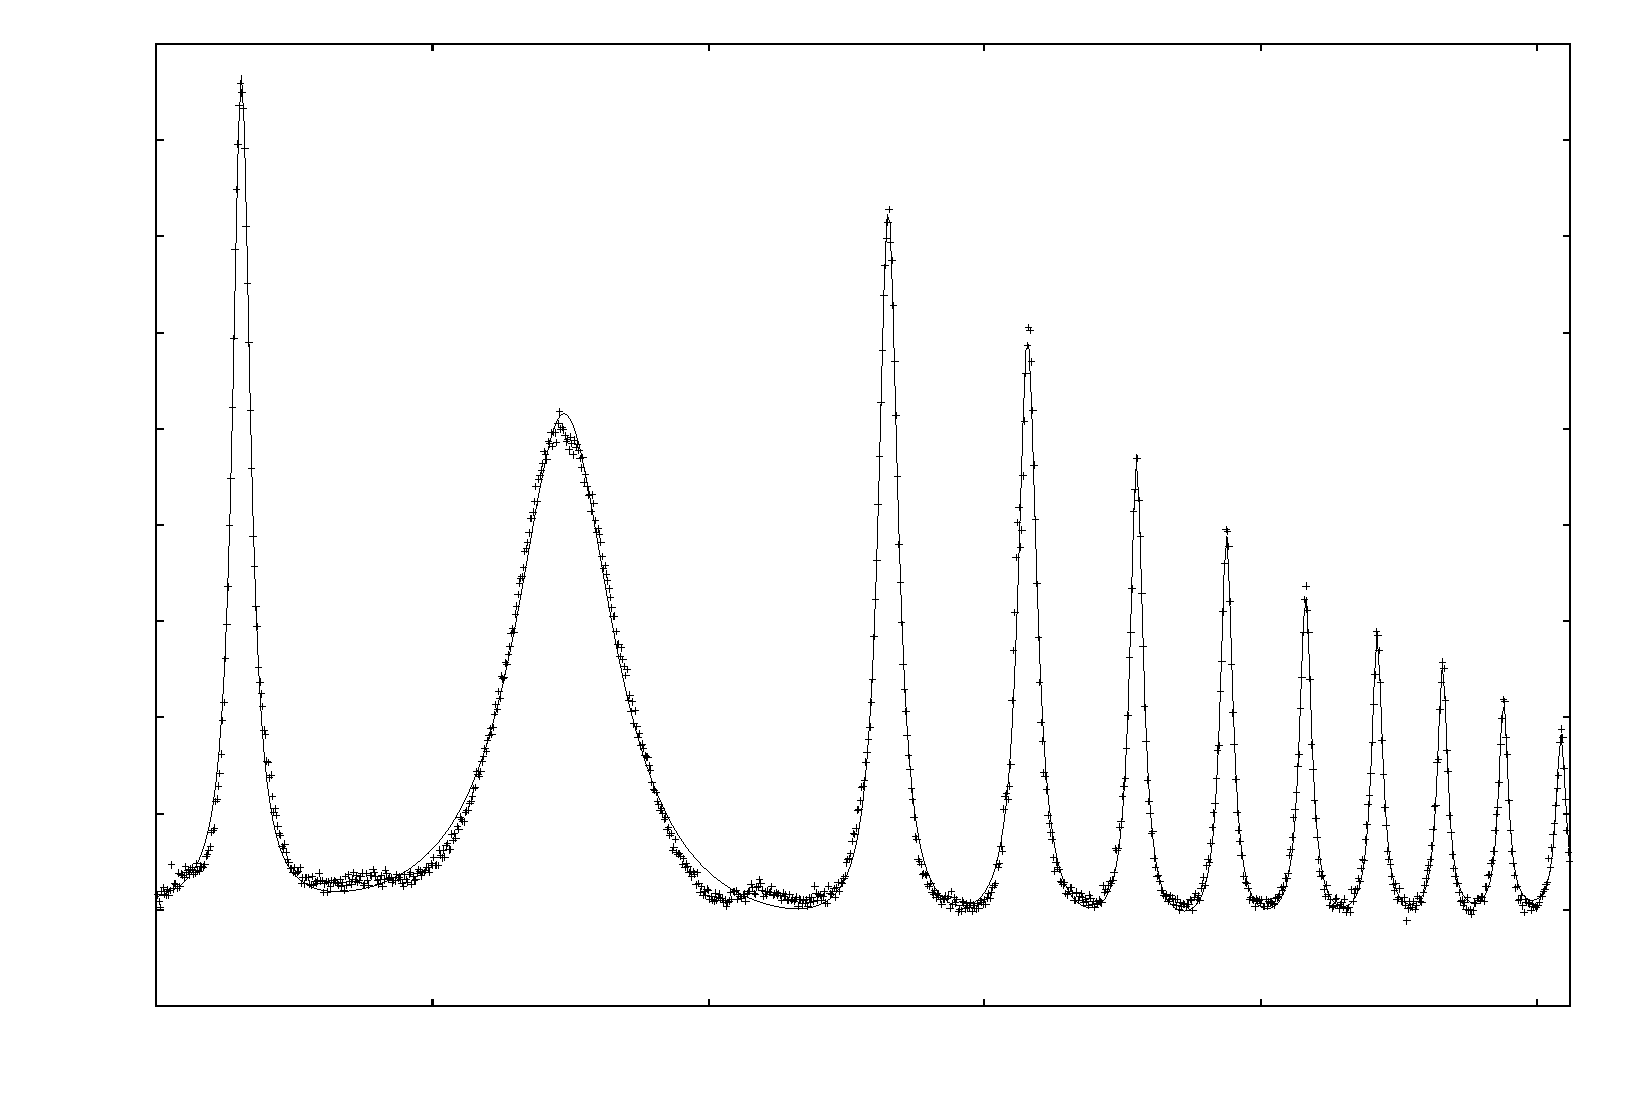
\includegraphics{plot-1}}%
    \gplfronttext
  \end{picture}%
\endgroup

%\end{landscape}
%
%\invisiblesection{Messprotokoll}
%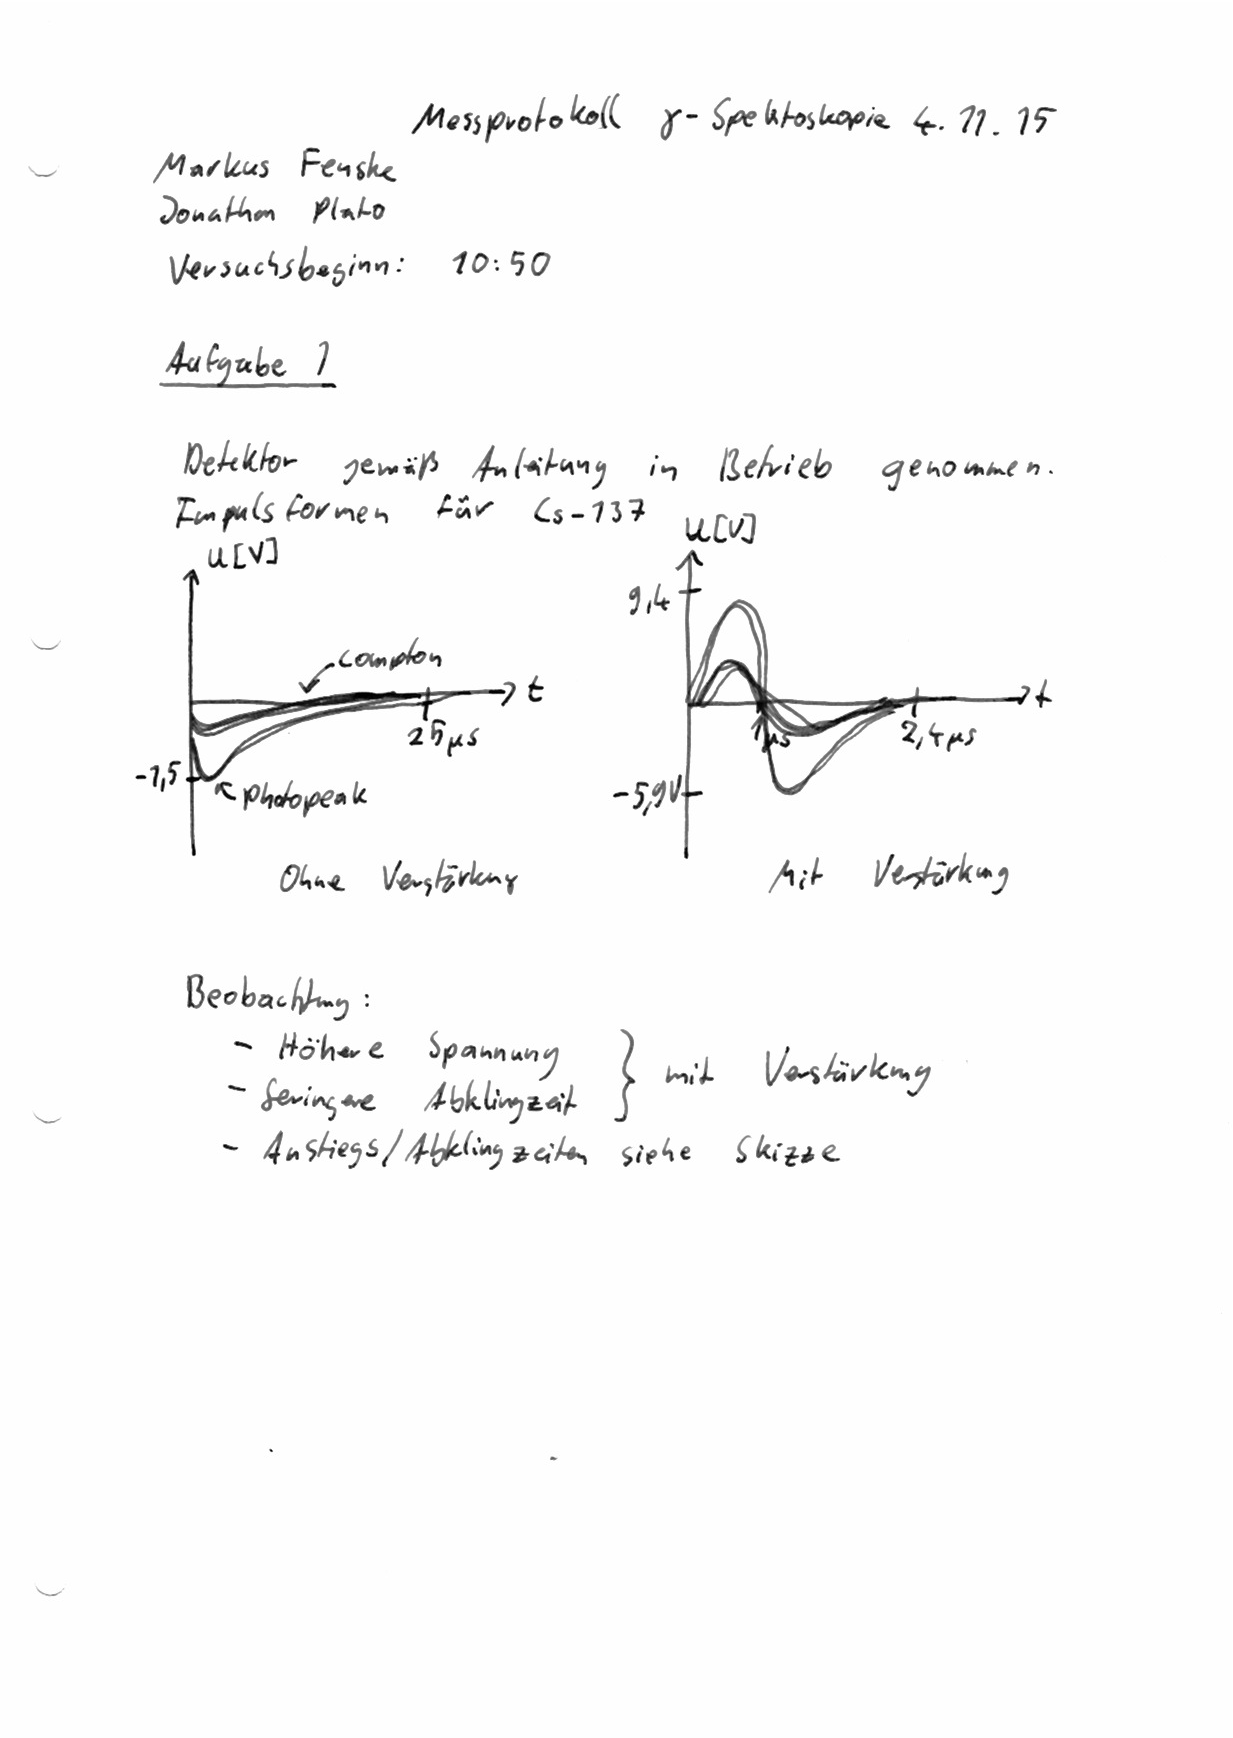
\includepdf[pages=-]{messprotokoll.pdf}
\end{document}
